\documentclass[t]{beamer}
\usepackage[T1]{fontenc}
\usepackage{lmodern}
\usepackage{amsmath}
\usepackage{amsfonts}
\usepackage{amssymb}
\usepackage{amsthm}
\usepackage{graphicx}
\usepackage{color}
\usepackage{xcolor}
\usepackage{url}
\usepackage{textcomp}
\usepackage{hyperref}
\usepackage{parskip}
\usepackage{minted}
\usepackage{multicol}
\usepackage{caption}

\usetheme[progressbar=frametitle]{metropolis}
\setbeamertemplate{frame numbering}[fraction]

\definecolor{vala}{rgb}{.482,.424,.639}
\definecolor{valadark}{rgb}{.241,.212,.320}
\setbeamercolor*{structure}{bg=vala!20,fg=vala}

\setbeamercolor*{palette primary}{use=structure,fg=white,bg=structure.fg}
\setbeamercolor*{palette secondary}{use=structure,fg=white,bg=structure.fg!75}
\setbeamercolor*{palette tertiary}{use=structure,fg=white,bg=structure.fg!50!black}
\setbeamercolor*{palette quaternary}{fg=white,bg=black}

\setbeamercolor{section in toc}{fg=black,bg=white}
%\setbeamercolor{alerted text}{use=structure,fg=structure.fg!50!black!80!black}

\setbeamercolor{titlelike}{parent=palette primary,fg=structure.fg!50!black}
\setbeamercolor{frametitle}{bg=vala!20!white,fg=vala!70!black}

%\setbeamercolor*{titlelike}{parent=palette primary}

\setbeamerfont{subsection in toc}{size=\small}

\hypersetup{
    colorlinks=true,
    linkcolor=valadark,
    citecolor=valadark,
    filecolor=valadark,
    urlcolor=vala
}

\newcommand{\fancyurl}[1]{\href{#1}{#1}}

\captionsetup{labelformat=empty}

\title{Improving App Development in Vala}
\author{Princeton Ferro}
\date{\today}

\newminted{json}{fontsize=\scriptsize, 
                   linenos,
                   numbersep=8pt,
                   gobble=4,
                   frame=lines,
                   bgcolor=bg,
                   framesep=3mm}

\begin{document}

\begin{frame}
    \titlepage
\end{frame}

\begin{frame}[c]{Outline}
    \tableofcontents
\end{frame}

%\section{What is Vala?}
%\begin{frame}[c]{What is Vala?}
%\begin{itemize}
%    \item The language of choice for eOS core libs and apps
%    \item Vala code $\rightarrow$ C $\rightarrow$ native code
%    \item Created as a GNOME subproject in 2006
%    \item Alternative to C, C++, and C\(\sharp\)
%    \item Selling points
%    \begin{itemize}
%        \item don't have to write boilerplate C/GObject code anymore
%        \item use high-level abstractions at near-zero cost
%        \item interops well with C libraries and GLib-based APIs
%    \end{itemize}
%\end{itemize}
%\end{frame}

%\begin{frame}[c]{Good things about Vala}
%    Vala is very good for UI programming:
%    
%    \begin{itemize}
%        \item Signals map nicely to UI events
%        \item Composite templates allow you to write your model and code together ({\small \texttt{[GtkTemplate]}}, {\small \texttt{[GtkChild]}}, {\small \texttt{[GtkCallback]}})
%        \item Async programming is easy $\rightarrow$ write responsive UIs with I/O event loops
%        \item Property binding + custom getters and setters $\rightarrow$ bind UI state to user preferences
%    \end{itemize}
%\end{frame}

%\begin{frame}[c]{Vala versus other languages}
%    Compared to \textbf{C\(\sharp\)}:
%    \begin{itemize}
%        \item Faster. No tracing GC or VM. (It's possible to compile C\(\sharp\) to native code but this isn't exposed in a practical way.)
%        \item Easier to debug
%        \item Better C interop
%    \end{itemize}
%    Compared to \textbf{Rust}:
%    \begin{itemize}
%        \item Simpler memory management, still affording you a decent amount of safety (as long as you don't use pointers)
%    \end{itemize}
%    Compared to \textbf{Swift}:
%    \begin{itemize}
%        \item Better C interop
%        \item Better support for async programming
%    \end{itemize}
%\end{frame}

%\begin{frame}[c]{However...}
%    Nevertheless, Vala isn't as popular, even for writing GNOME apps. Why?
%\end{frame}

%\begin{frame}[c]{The right language}
%    A language is more than its \textit{features}.
%    
%    A bad language can fail, but a good language does not necessarily succeed.
%    
%    Java remains a popular (bad) language. Why?
%    
%    Good tooling. Good support.
%    
%    A language is an \textit{ecosystem}.
%    
%    If we want to make Vala better, we have to improve the Vala ecosystem.
%    
%    We should start with tooling.
%\end{frame}

\section{A language server for Vala}
\begin{frame}[c]{A language server for Vala}
    A language server is the first big step to improving the Vala developer experience.
    
    \begin{itemize}
        \item Language servers provide code intelligence.
        \item Code intelligence helps you iterate faster.
        \item Iterating faster means you develop higher-quality apps.
    \end{itemize}
\end{frame}

%\section{A language server for Vala}
%\begin{frame}[c]{A language server for Vala}
%    Some brief history:
%    \begin{itemize}
%        \item Started development in summer 2017
%        \item Hiatus (school)
%        \item Development picked up in winter 2018
%        \item Hiatus (school)
%        \item Development significantly picked up again in late 2019
%    \end{itemize}
%\end{frame}

\begin{frame}[c]{Precursors}
    \begin{itemize}
        \item Valama IDE
        \item vala-pack (GNOME Builder)
        \item gedit-code-assistance
        \item Anjuta
    \end{itemize}
    
    These weren't very good.
    
    If you wanted Vala to be supported on $N$ editors, you had to write $N$ plugins.
\end{frame}

\begin{frame}[c]{The Language Server Protocol}
    Allows you to write \textit{one} language server for $N$ editors.
    
    Defines how an editor should ask a language server for diagnostics, completion suggestions, etc.
    
    Very flexible--during handshake, server and client advertise what methods they support.
\end{frame}

\subsection{Architecture}
\begin{frame}[c]{Architecture}
    \begin{figure}
        \begin{center}
            \def\svgwidth{\columnwidth}
            \input{res/vls-architecture.pdf_tex}
            \caption{Architecture of VLS}
        \end{center}
    \end{figure}
\end{frame}

\begin{frame}[c]{Architecture}    
    Initial problems:
    \begin{itemize}
        \item Plugging compiler memory leaks
        \begin{itemize}
            \item Reduced average memory consumption from a few GB to a few hundred MB
        \end{itemize}
        \item Recovering from syntax errors
    \end{itemize}
\end{frame}

\begin{frame}[c]{Architecture}
    User interaction must be fast:
    \begin{itemize}
        \item Delay context updates while user is typing
        \item Use backwards parser to extract simple expressions for rapid completion
    \end{itemize}
\end{frame}

\begin{frame}[c]{Architecture}
    The server--not the plugin--should know as much about the build system as possible, since we don't want to reimplement project management across $N$ editors.
\end{frame}

\begin{frame}[c]{Architecture}
    \begin{itemize}
        \item Integrate with Meson build system
            \begin{itemize}
                \item Has a friendly introspection API
                \item Vala is a first-class citizen
                \item Used by >95\% of Vala projects
            \end{itemize}
        \item Autotools introspection is too complex, not worth the effort
        \item CMake introspection API is okay but Vala targets aren't recognized
        \begin{itemize}
            \item We'd first need to write a CMake plugin for Vala (and convince people to use it)
        \end{itemize}
    \end{itemize}
\end{frame}

\begin{frame}[c]{Architecture}
    Navigation:
    \begin{itemize}
        \item Show references
        \item Go to implementation(s)
        \item Go to base/hidden method
    \end{itemize}
    
    Code refactoring:
    \begin{itemize}
        \item Rename symbol
    \end{itemize}
\end{frame}

\begin{frame}[c]{Architecture}
    For documentation, we read the GObject Introspection files--which usually come installed with the library--and parse them according to the GTK-Doc\footnote{\fancyurl{https://developer.gnome.org/gtk-doc-manual/stable/}} and ValaDoc\footnote{\fancyurl{https://valadoc.org/markup.htm}} markup languages.
    
    The GTK-Doc comments are usually written for the C version of the API. Therefore, in a second step, we map the C identifiers to Vala identifiers. This produces documentation that more closely resembles Vala code.
\end{frame}

\subsection{Editor support}
\begin{frame}[c]{Editor support}
    Today you can get code intelligence for Vala in a lot of editors, thanks to plugins and built-in support.
    
    \begin{itemize}
        \item Visual Studio Code
        \item GNOME Builder
        \item Neovim and vim8
        \item Kate
        \item Emacs
        \item Sublime Text
    \end{itemize}
\end{frame}

\begin{frame}[c]{Editor support}
    Visual Studio Code
    \begin{itemize}
        \item Install \href{https://marketplace.visualstudio.com/items?itemName=prince781.vala}{Vala plugin}
    \end{itemize}
    
    GNOME Builder
    \begin{itemize}
        \item Bundled with VLS
        \item Enable "Vala Language Server" and disable "GVLS"
    \end{itemize}
\end{frame}

\defverbatim[colored]\exampleCode{
\begin{jsoncode}
        "languageserver": {
            "vala": {
                "command": "vala-language-server",
                "filetypes": ["vala", "genie"]
            }
        }
\end{jsoncode}
}

\begin{frame}[c]{Editor support}
    vim8/neovim
    \begin{itemize}
        \item Install \href{https://github.com/neoclide/coc.nvim}{coc.nvim}
        \item Add this to your config (\texttt{:CocConfig})
        \item Works well with \href{https://github.com/liuchengxu/vista.vim}{vista.vim} plugin.
    \end{itemize}
    \exampleCode
    
    Or you can install \href{https://github.com/neovim/nvim-lspconfig/blob/f81570d1288fd974098e0f311f728469ca919155/lua/lspconfig/vala\_ls.lua}{nvim-lspconfig} for neovim.
\end{frame}

\begin{frame}[c]{Editor support}
    Kate
    \begin{itemize}
        \item Enable built-in LSP plugin
    \end{itemize}
    
    Emacs
    \begin{itemize}
        \item Install \href{https://emacs-lsp.github.io/lsp-mode/page/lsp-vala/}{lsp-mode}
    \end{itemize}
\end{frame}

\defverbatim[colored]\exampleCode{
\begin{jsoncode}
        "clients": {
            "vala-language-server": {
                "command": [
                    "/usr/bin/vala-language-server"
                ],
                "selector": "source.vala | source.genie"
            },
        }
\end{jsoncode}
}

\begin{frame}[c]{Editor support}
    Sublime Text
    \begin{itemize}
        \item Install the \href{https://packagecontrol.io/packages/Vala-TMBundle}{Vala-TMBundle} and \href{https://github.com/sublimelsp/LSP}{LSP} packages
        \item Add config below to \texttt{LSP.sublime-settings}
        \item \texttt{Tools > LSP > Enable Language Server Globally... > vala-language-server}
    \end{itemize}
    \exampleCode
\end{frame}

\subsection{Future plans}
\begin{frame}[c]{Future plans}
    What's next?
\end{frame}

\begin{frame}[c]{Responsiveness}
    For large projects (> 20000 lines), VLS is slow.
    
    Off-main-thread compilation or incremental recompilation?
    \begin{itemize}
        \item Threaded compilation: fast and "simple", but uses much more memory (code context duplication)
        \item Incremental recompilation: less memory (reuse existing code context), faster, but is much more complex to implement
        \begin{itemize}
            \item Relies on the observation that most of the code context is unchanged as you type
            \item Corner case--refactoring commonly-used symbols
        \end{itemize}
    \end{itemize}
\end{frame}

\begin{frame}[c]{Code refactoring}
    Things on my radar:
    
    \begin{itemize}
        \item Organize imports
        \item Extract to variable/method/...
        \item Inline
        \item Change signature of a method
        \item Delete method
    \end{itemize}
\end{frame}

\begin{frame}[c]{Completion}  
    There are a \emph{lot} of additional cases to be covered. We have multiple issues tracking this.\footnote{\fancyurl{https://github.com/Prince781/vala-language-server/milestone/2}}
    
    In general, we want code suggestions to be context-sensitive, and to work without configuration.
\end{frame}

\begin{frame}[c]{Smart method completion}
    For example, we want to complete a method. Do we do this:
    
    \texttt{method (...args)}
    
    or this:
    
    \texttt{method(...args)}
    
    Most projects use the first style, but a few notable ones (Geary) use the second.
    
    Rather than expose a configuration option, we should understand the coding style and always do the right thing.
\end{frame}

\begin{frame}[c]{Global completion}
    Show symbols within namespaces we haven't imported, and import the appropriate namespace for the selected symbol.
\end{frame}


\section{Improving Vala}
\begin{frame}[c]{Improving Vala}
    A year and a half ago, none of this was possible. Writing Vala was a bare experience. 
    
    Things are better now, but there's still much room for improvement.
    
    Vala still needs better tooling and better infrastructure.
    
    This is key to improving the Vala ecosystem.
\end{frame}

\begin{frame}[c]{Improving Vala}
    Lets examine other areas:
    \begin{itemize}
        \item Tooling
        \begin{itemize}
            \item Static analysis
            \item Linting and Formatting
            \item Templating
            \item Dependency management
        \end{itemize}
        \item Website
        \item Documentation
        \item Community
    \end{itemize}
\end{frame}

\subsection{Static analysis}
\begin{frame}[c]{Static analysis}
    It would be nice to have something like Clang's \texttt{scan-build} or GCC's \texttt{-fanalyzer} for Vala.
    
    These tell you about deeper errors in your code and usually don't care about showing you some false positives. (For example, null pointer access or use-after-free.)
    
    For Vala we could have reference cycle detection.
\end{frame}

\defverbatim[colored]\exampleCodeBad{
\begin{minted}[fontsize=\scriptsize]{vala}
class List<T> {
    public T data;
    public List<T>? prev;
    public List<T>? next;
    
    public List<T> add (T data) {
        next = new List<T> () {
            data = data,
            prev = this
        };
        return next;
    }
}
\end{minted}
}

\defverbatim[colored]\exampleCodeFixed{
\begin{minted}[fontsize=\scriptsize]{vala}
class List<T> {
    public T data;
    public weak List<T>? prev;
    public List<T>? next;
    
    public List<T> add (T data) {
        next = new List<T> () {
            data = data,
            prev = this
        };
        return next;
    }
}
\end{minted}
}

\begin{frame}[c]{Static analysis}
    Reference cycle detection could give warnings when using cyclic data structures improperly.
    
    \begin{multicols}{2}
        Bad:
        
        \exampleCodeBad
        
        \columnbreak
        
        Good:
        
        \exampleCodeFixed
    \end{multicols}
\end{frame}

\defverbatim[colored]\exampleCodeBad{
\begin{minted}[fontsize=\scriptsize]{vala}
class Zombie {
    public bool sort_ascend;
    public int age { get; private set; }
    public Gee.Set<Zombie> children { get; private set; }

    public Zombie (int age) {
        this.age = age;
        children = new Gee.TreeSet<Zombie> (
            (a, b) => sort_ascend ? a.age - b.age : b.age - a.age
        );
    }
}
\end{minted}
}

\defverbatim[colored]\exampleCodeFixed{
\begin{minted}[fontsize=\scriptsize]{vala}
class Zombie {
    public bool sort_ascend;
    public int age { get; private set; }
    public Gee.Set<Zombie> children { get; private set; }
    static CompareDataFunc<Zombie> make_compare (Zombie _self) {
        weak Zombie self = _self;
        return (a, b) =>
            self.sort_ascend ? a.age - b.age : b.age - a.age;
    }
    public Zombie (int age) {
        this.age = age;
        children = new Gee.TreeSet<Zombie> (make_compare (this));
    }
}
\end{minted}
}

\begin{frame}{Static analysis}
    Or when creating circular references in subtle ways...
    
    \exampleCodeBad
    
    Closure holds strong reference to \texttt{this}.
\end{frame}

\begin{frame}{Static analysis}
    Or when creating circular references in subtle ways...
    
    \exampleCodeFixed
    
    Closure now holds a weak reference to \texttt{this}.
\end{frame}

\subsection{Linting and Formatting}
\begin{frame}[c]{Linting and Formatting}
    Linters suggest fixes to code structure and semantics. They catch errors and unintended behavior.
    
    Formatters are basically code "prettifiers."
    
    Vala has \texttt{vala-lint}, which is mostly a code prettifier analogous to \texttt{rustfmt}.
    
    We also need something like \texttt{rust-clippy}.
\end{frame}

\defverbatim[colored]\exampleCode{
\begin{minted}[fontsize=\scriptsize]{rust}
fn main() {
    let a = 1.231f32;
    let b = 1.232f32;

    if a == b {
        print!("a == b");
    } else {
        print!("a != b");
    }
}
\end{minted}
}

\begin{frame}[c]{Linting}
    For example, \texttt{rust-clippy} has hundreds of lints, can catch common programming mistakes, and offers suggestions for fixing them.
    
    A sample:
    
    \exampleCode
\end{frame}

\defverbatim[colored]\exampleCode{
\begin{minted}[fontsize=\scriptsize,breaklines=true]{text}
% clippy-driver comparef32.rs
error: strict comparison of `f32` or `f64`
 --> comparef32.rs:5:8
  |
5 |     if a == b {
  |        ^^^^^^ help: consider comparing them within some margin of error: `(a - b).abs() < error_margin`
  |
  = note: `#[deny(clippy::float_cmp)]` on by default
  = note: `f32::EPSILON` and `f64::EPSILON` are available for the `error_margin`
  = help: for further information visit
https://rust-lang.github.io/rust-clippy/master/index.html#float_cmp

error: aborting due to previous error
\end{minted}
}

\begin{frame}[c]{Linting}
    \exampleCode
\end{frame}

\subsection{Templating}
\begin{frame}[c]{Templating}
    Templates allow developers to zoom past project setup and jump straight to writing code.
    
    For C$\sharp$, there's officially \texttt{dotnet new}, which allows you to initialize a new project from a collection of community-made templates.
    
    Other languages have similar unofficial tools.
\end{frame}

%\defverbatim[colored]\exampleCode{
%\begin{minted}[fontsize=\scriptsize]{text}
%% dotnet new
%Templates                                     Short Name     ...
%--------------------------------------------  -------------- ---
%Console Application                           console        ...
%Class library                                 classlib      
%Worker Service                                worker        
%Unit Test Project                             mstest        
%NUnit 3 Test Project                          nunit         
%NUnit 3 Test Item                             nunit-test    
%xUnit Test Project                            xunit         
%Razor Component                               razorcomponent
%Razor Page                                    page          
%MVC ViewImports                               viewimports   
%MVC ViewStart                                 viewstart     
%Blazor Server App                             blazorserver  
%Blazor WebAssembly App                        blazorwasm    
%ASP.NET Core Empty                            web           
%ASP.NET Core Web App (Model-View-Controller)  mvc           
%ASP.NET Core Web App                          webapp
%...
%\end{minted}
%}

%\begin{frame}[c]{Templating}
%    \exampleCode
%\end{frame}

\defverbatim[colored]\exampleCode{
\begin{minted}[fontsize=\scriptsize]{text}
% valdo
Available templates:
--------------------
new - a bare app, with minimal dependencies
lib - a bare library with minimal dependencies
gtk - a starter GTK3 app
\end{minted}
}

\begin{frame}[c]{Templating}
    Recently I introduced \texttt{valdo}\footnote{\fancyurl{https://github.com/Prince781/valdo}} with the same idea.
    
    \exampleCode
    
    I think it would be good if this takes off.
    
    I encourage anyone with ideas to submit PRs for new templates.
\end{frame}

\subsection{Dependency management}
\begin{frame}[c]{Dependency management}
    Rust/JS/Go/C$\sharp$ dependencies are per-project, statically linked in or bundled.
    
    Vala dependencies are system-wide, dynamically linked in.
    
    How to bridge the gap?
\end{frame}

\subsection{Website}
\begin{frame}[c]{Website}
    \begin{figure}
        \begin{center}
            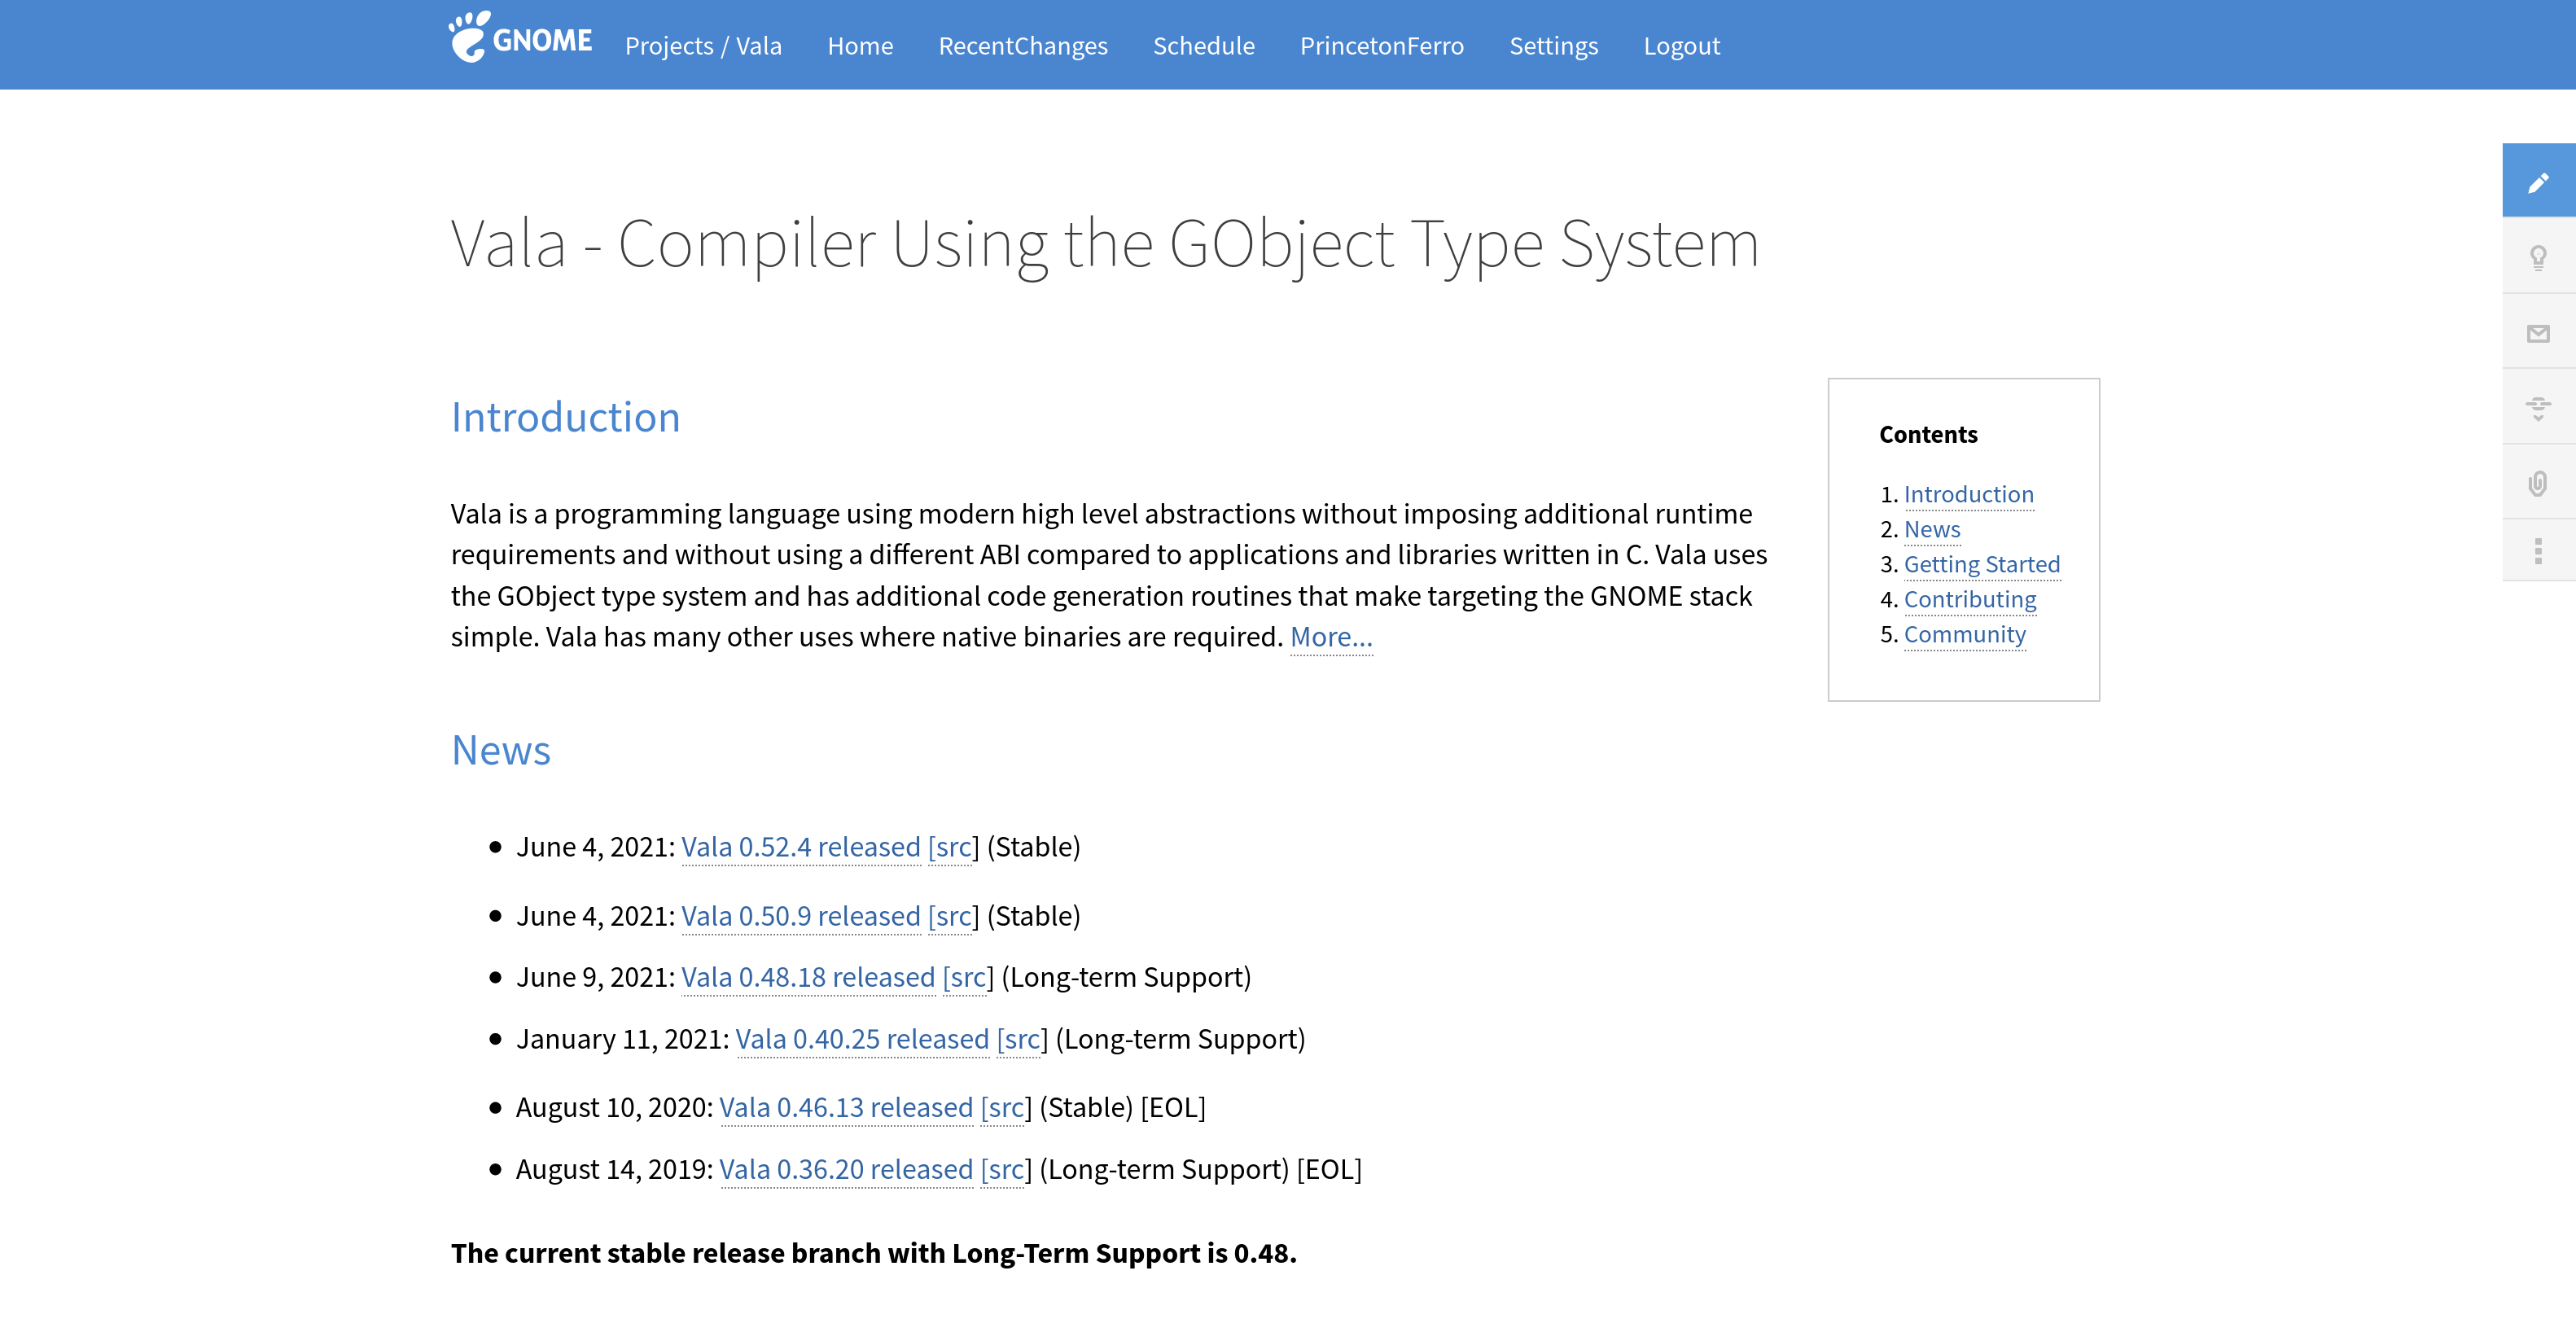
\includegraphics[scale=.1]{res/Screenshot 2021-06-22 at 12-08-52 Projects Vala - GNOME Wiki.png}
            \caption{The current website\footnote{{\scriptsize \fancyurl{https://wiki.gnome.org/Projects/Vala}}} isn't very friendly to newcomers}
        \end{center}
    \end{figure}
\end{frame}

\begin{frame}[c]{Website}
    \begin{figure}
        \begin{center}
            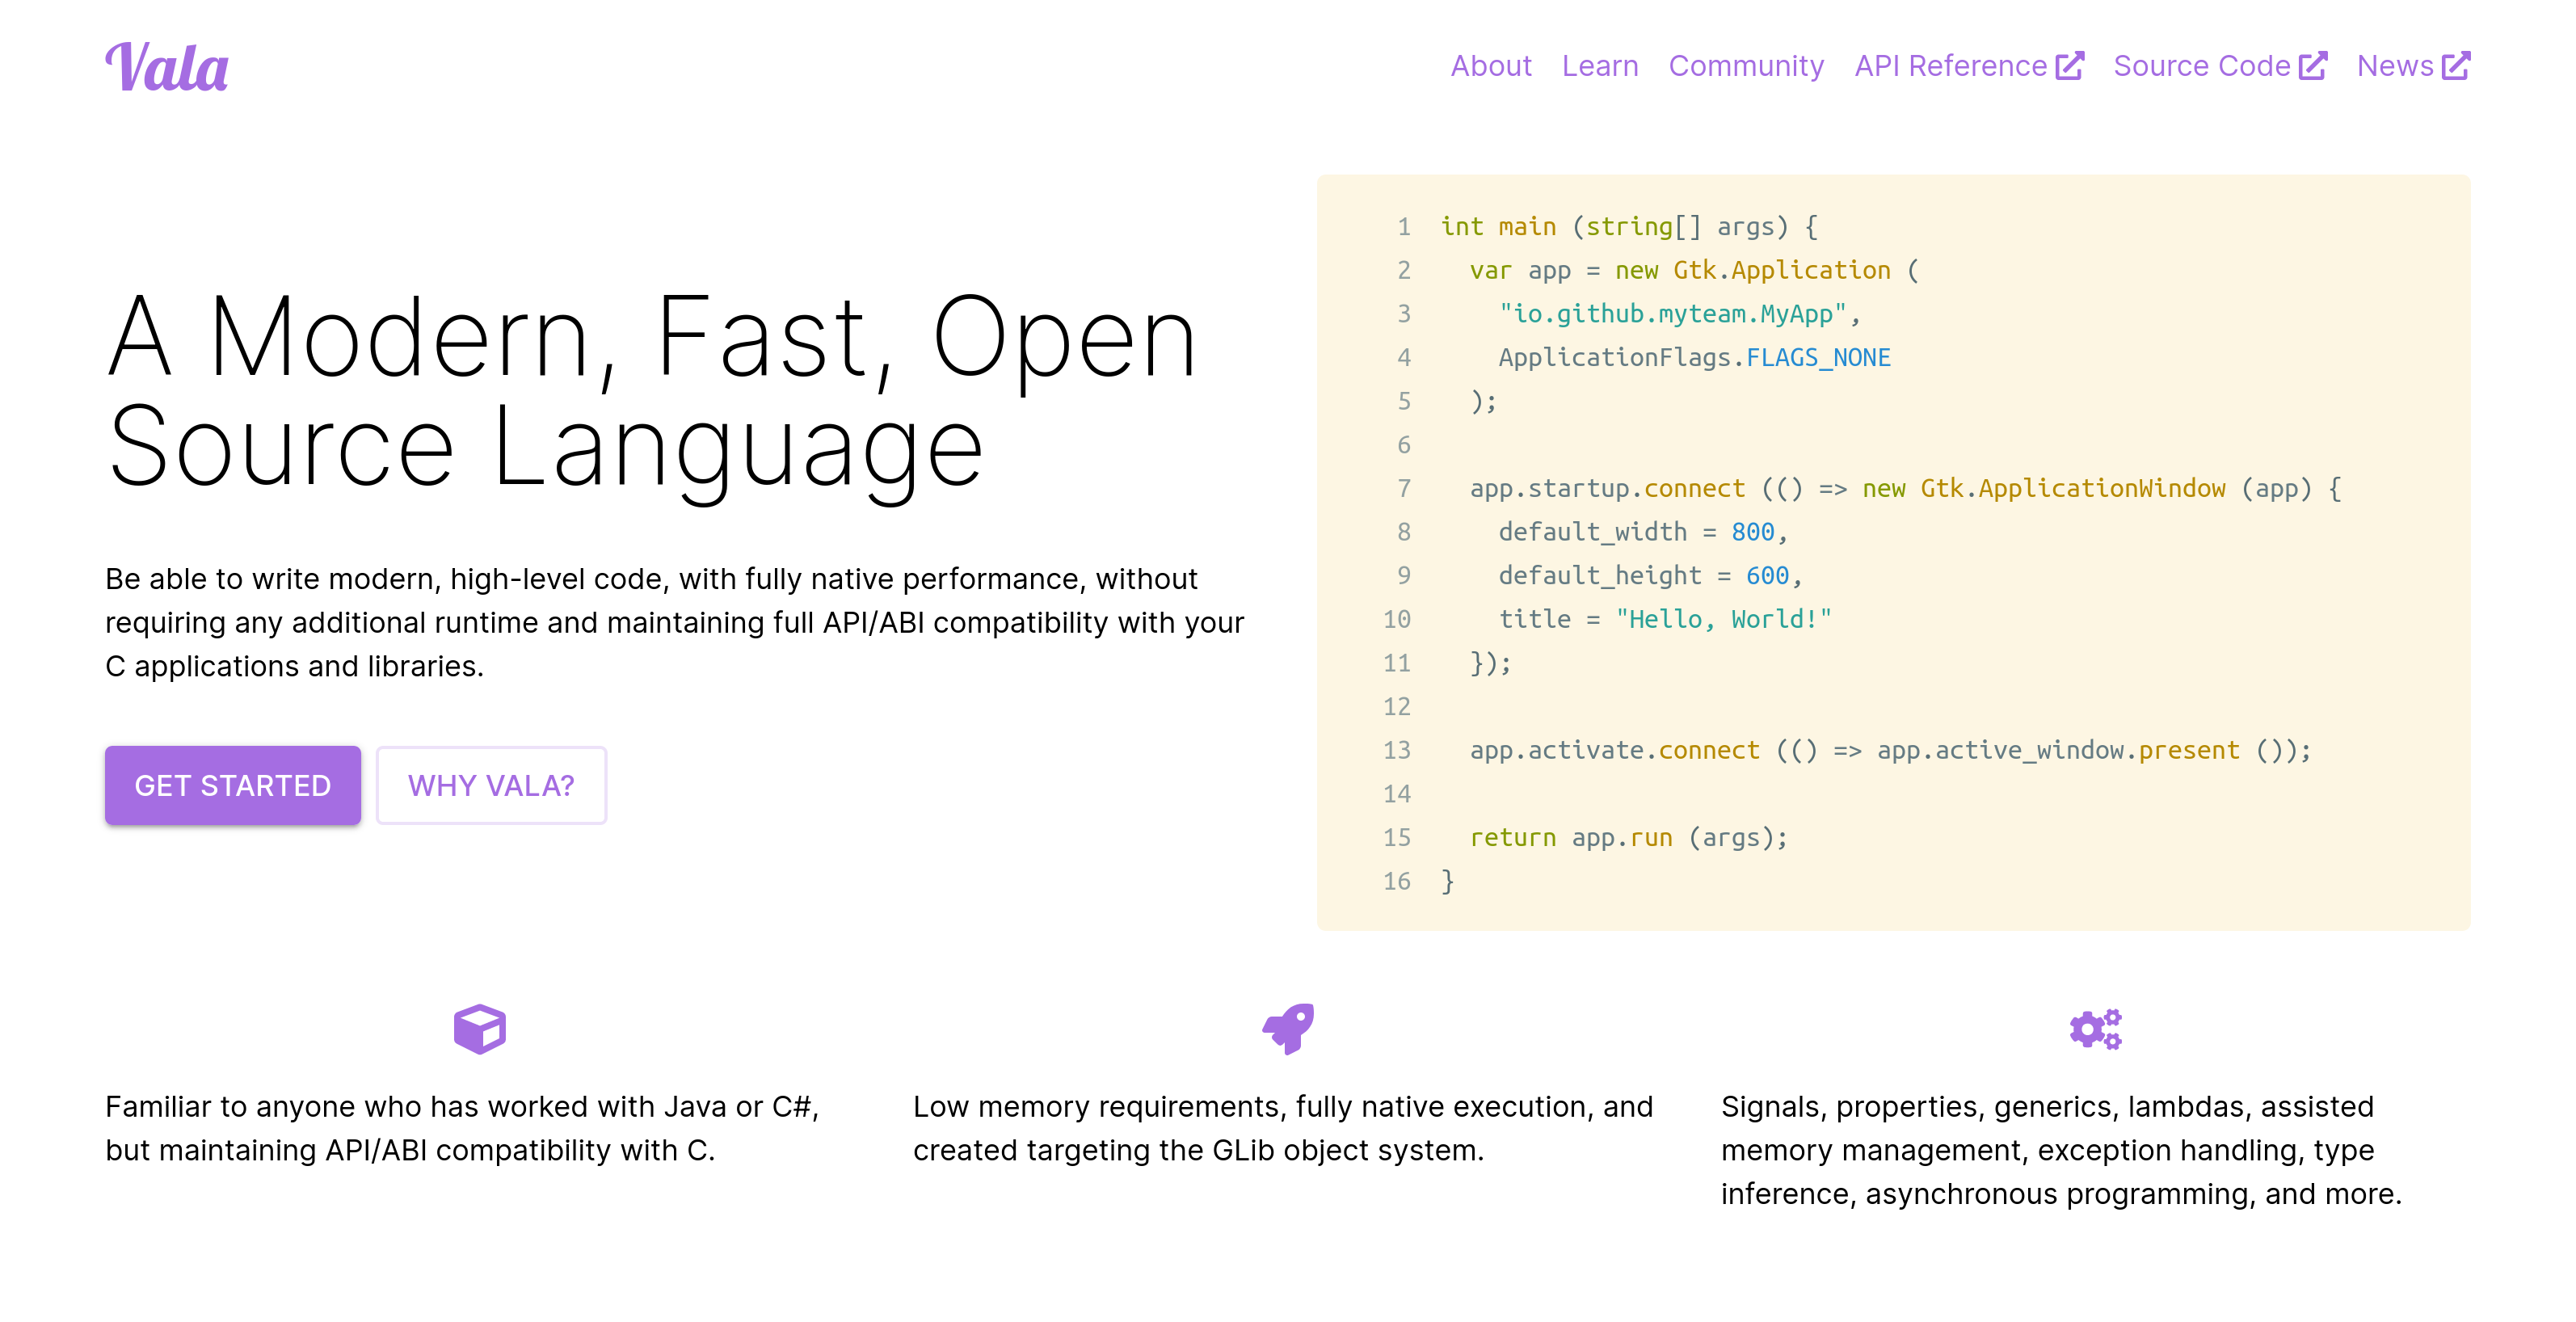
\includegraphics[scale=.1]{res/Screenshot 2021-06-22 at 12-17-51 Vala Programming Language.png}
            \caption{Proposal for a new website\footnote{{\scriptsize \fancyurl{https://github.com/nahuelwexd/vala-website}}} at \href{https://vala-lang.org}{vala-lang.org}}
        \end{center}
    \end{figure}
\end{frame}

\subsection{Documentation}
\begin{frame}[c]{Documentation}
    \href{https://valadoc.org}{valadoc.org} is very good, but it could be better
    
    It's mostly an API browser with some code snippets.
    
    There are existing tutorials out there. Can we centralize everything (APIs and tutorials) into one website?
    
    \begin{itemize}
        \item \fancyurl{https://naaando.gitbooks.io/the-vala-tutorial/content/en/1-introduction/what-is-vala.html}
        \item \fancyurl{https://wiki.gnome.org/Projects/Vala/Tutorial}
        \item \fancyurl{https://developer.gnome.org/gnome-devel-demos/stable/beginner.vala.html}
    \end{itemize}
\end{frame}

\begin{frame}[c]{Community}
    \texttt{\#vala}\footnote{\fancyurl{irc://irc.gnome.org/vala}} is nice, but IRC isn't for everyone.
    
    Recently a Vala Discord\footnote{\fancyurl{https://discord.gg/YFAzjSVHt7}} has been created. It's become quite popular. I encourage people to join!
    
    Also a Twitter account\footnote{\fancyurl{https://twitter.com/vala\_lang}} has been created to promote the language. Consider following it.
    
    Thanks for listening!
\end{frame}

\end{document}